To evaluate how the different models were able to perform, I prepared the resulting data in a few different ways. First, I will compare the training histories for the training and validation loss in \autoref{fig:history_all}. Afterwards I will inspect the most accurate of all deep models ResNet152V2 and compare it with the basic CNN and its predictions. At the end, in \autoref{tab:results_table} I set side by side all key metrics of the best performing models.

\subsubsection{Training History Comparison}

Training resulted in many different outcomes depending on the model. To help compare the training history of all models consider \autoref{fig:history_all}. The training history of both the training and validation loss is shown in one plot each for easy comparison. Because of the many spikes seen in training, the losses are smoothed using the simple moving average (SME) \eqref{rol_mean} with $k = 100$ entries taken into account for smoothing a single value.

\begin{figure}[H]
\begin{subfigure}{.5\textwidth}
    \centering
    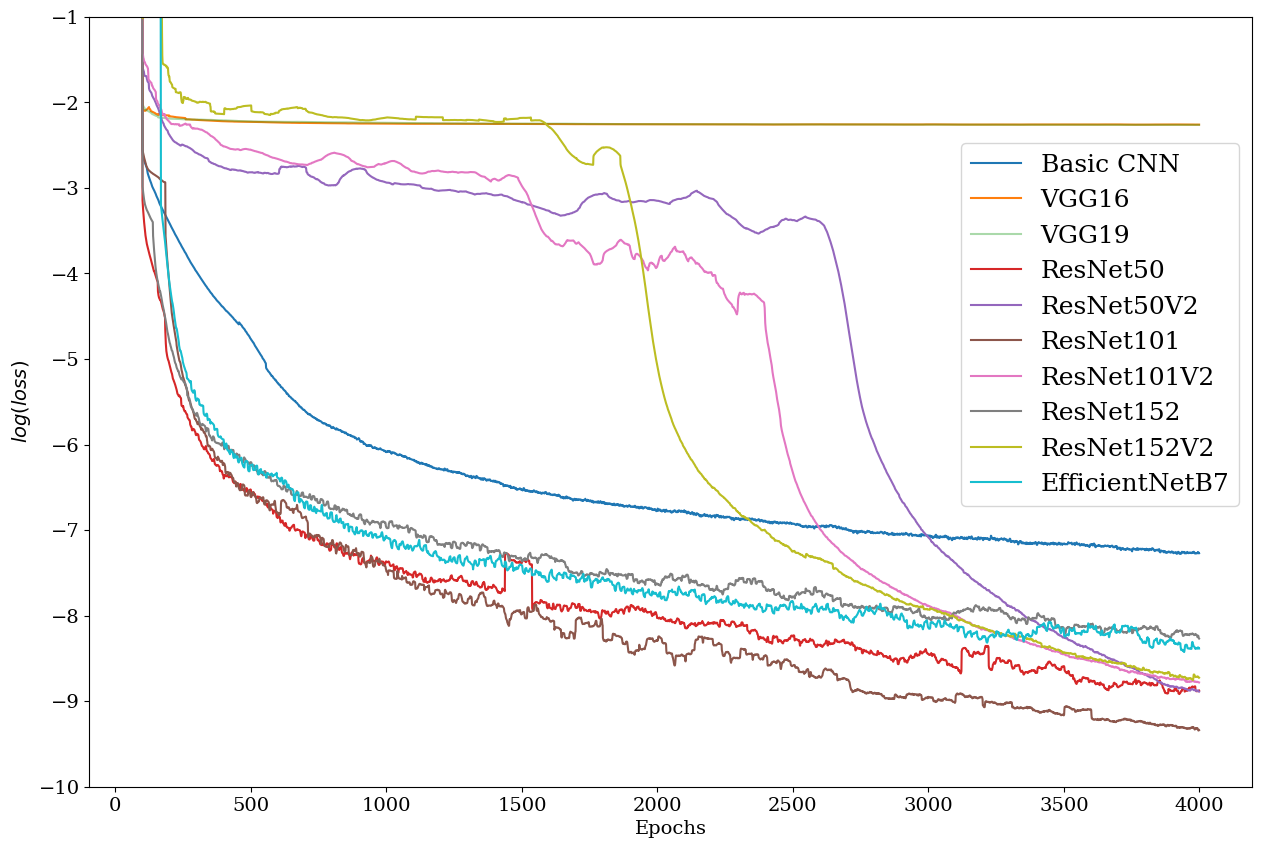
\includegraphics[width=\linewidth]{images/Chapter4/Results/tr_loss_hist.png}
    \caption{Training loss for all models}
    \label{fig:history_all_training_loss}
\end{subfigure}
\begin{subfigure}{.5\textwidth}
    \centering
    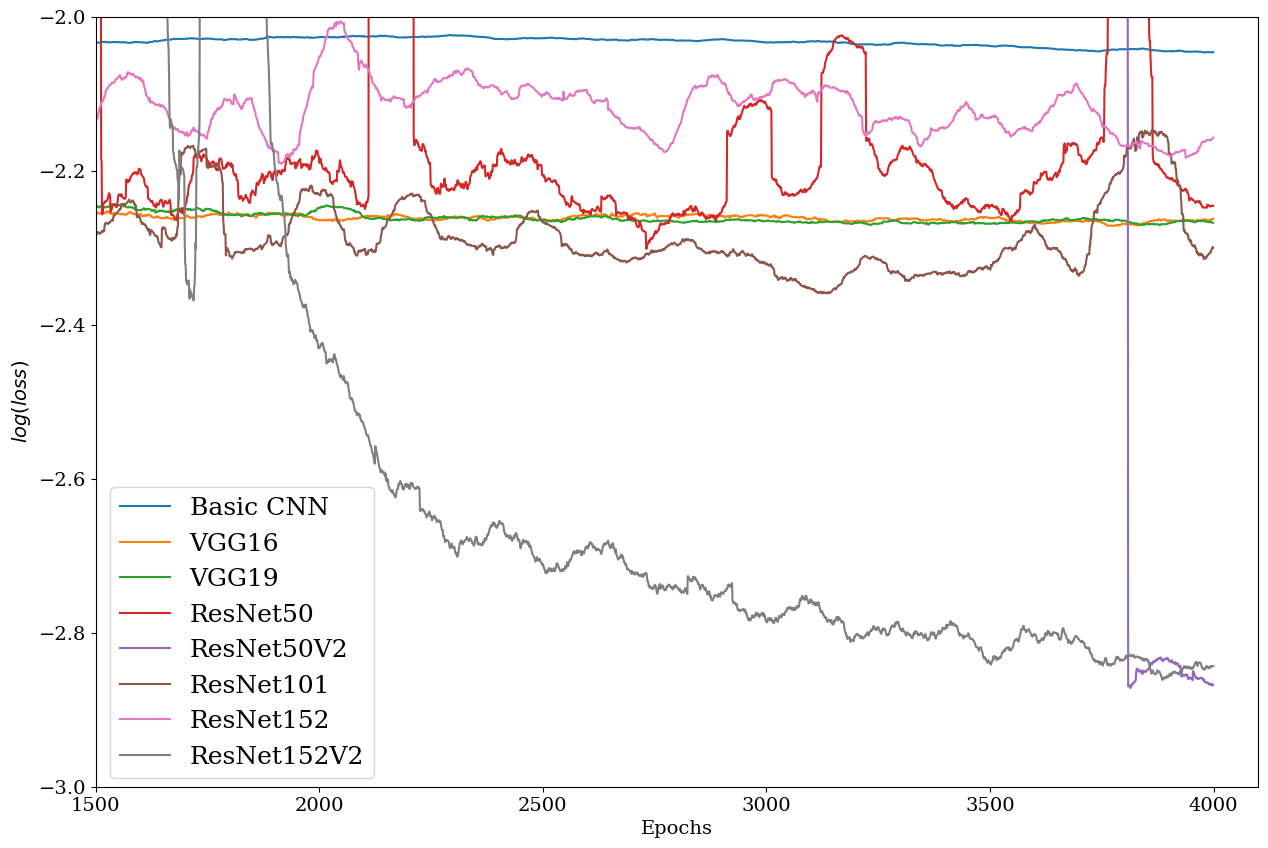
\includegraphics[width=\linewidth]{images/Chapter4/Results/val_loss_hist.png}
    \caption{Validation loss for all models}
    \label{fig:history_all_validation_loss}
\end{subfigure}
\caption{Training loss history for all deep models gives a good comparison of different learning outcomes. The VGG models were not able to predict accurately and thus their training loss could not improve over the 4000 epochs. The other models either improved very quickly at the beginning or were able to find helpful features later in training. For the validation loss (\textit{right}) only the best seven models are shown for easier comparison. Remember that the basic CNN shown in this graphic is not the best performing model because it only trained for around 100 epochs. Instead the overfitted model from \autoref{fig:basic_cnn_overf} is shown to compare it to the deep models. The training and validation loss histories are smoothed using the simple moving average (SMA) \eqref{rol_mean} with $k = 100$ entries taken for smoothing.}
\label{fig:history_all}
\end{figure}

Especially the two best performing deep models ResNet50V2 and ResNet152V2 are clearly separated from the other models in validation loss (see \autoref{fig:history_all_validation_loss}) with values around $-2.9$. One thing I don't yet understand is that the training loss of the overfitted baseline network is considerably higher ($\sim -7$) than the training loss of the other deep models ($< -8 $) considering the way more accurate predictions on the training set for the baseline model. I do not know where this discrepancy comes from but it would be very interesting to investigate this further. 

\subsubsection{Best Performing Deep CNN vs. Basic CNN}
ResNet152V2 was able to get closest to the basic CNN in terms of validation loss and standard deviation on the test set with $\sigma = 0.134$. The biggest difference between these two models is in the expected value $\mu$, where the basic CNN was able to perform really well with $\mu \sim 0$. ResNet152V2 struggled a little bit with predicting smaller values than the true masses which resulted in a $\mu$ value of $0.055$. Obviously, the deep model is no way near as efficient as the basic CNN with a training time of roughly one day for each run of 4000 epochs while the basic CNN only takes minutes to get more accurate predictions. 

\begin{figure}[H]
\begin{subfigure}{.5\textwidth}
    \centering
    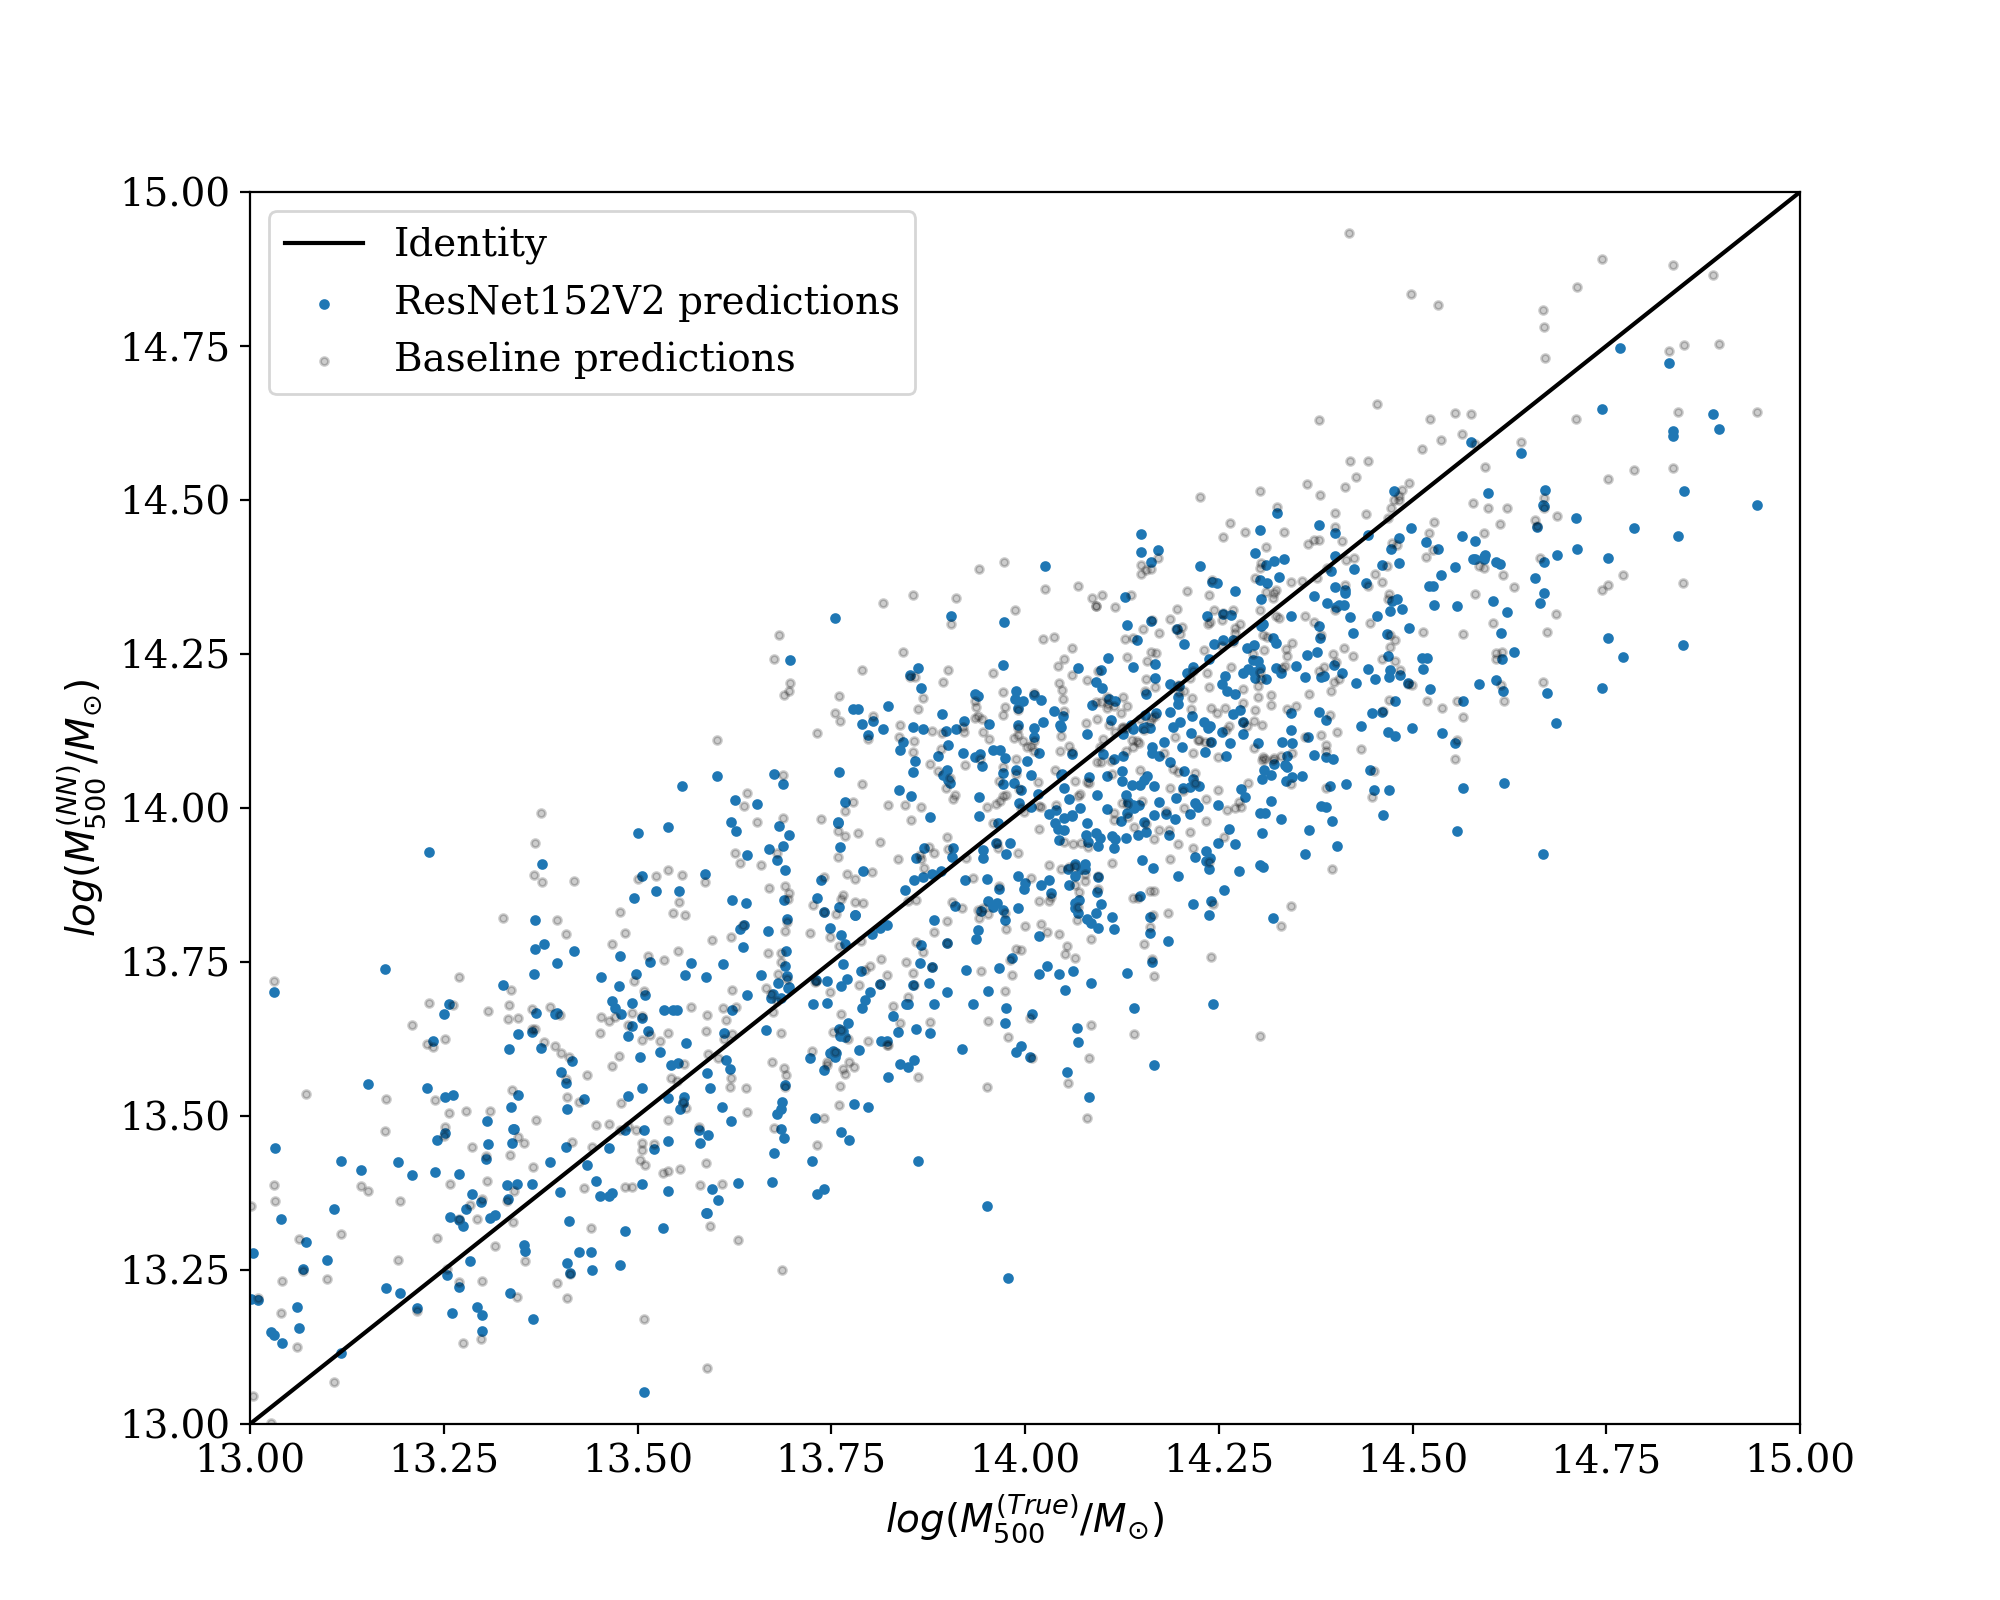
\includegraphics[width=\linewidth]{images/Chapter4/Results/test_ResNet152V2_scatter.png}
    \label{fig:test_ResNet152V2_scatter}
\end{subfigure}
\begin{subfigure}{.5\textwidth}
    \centering
    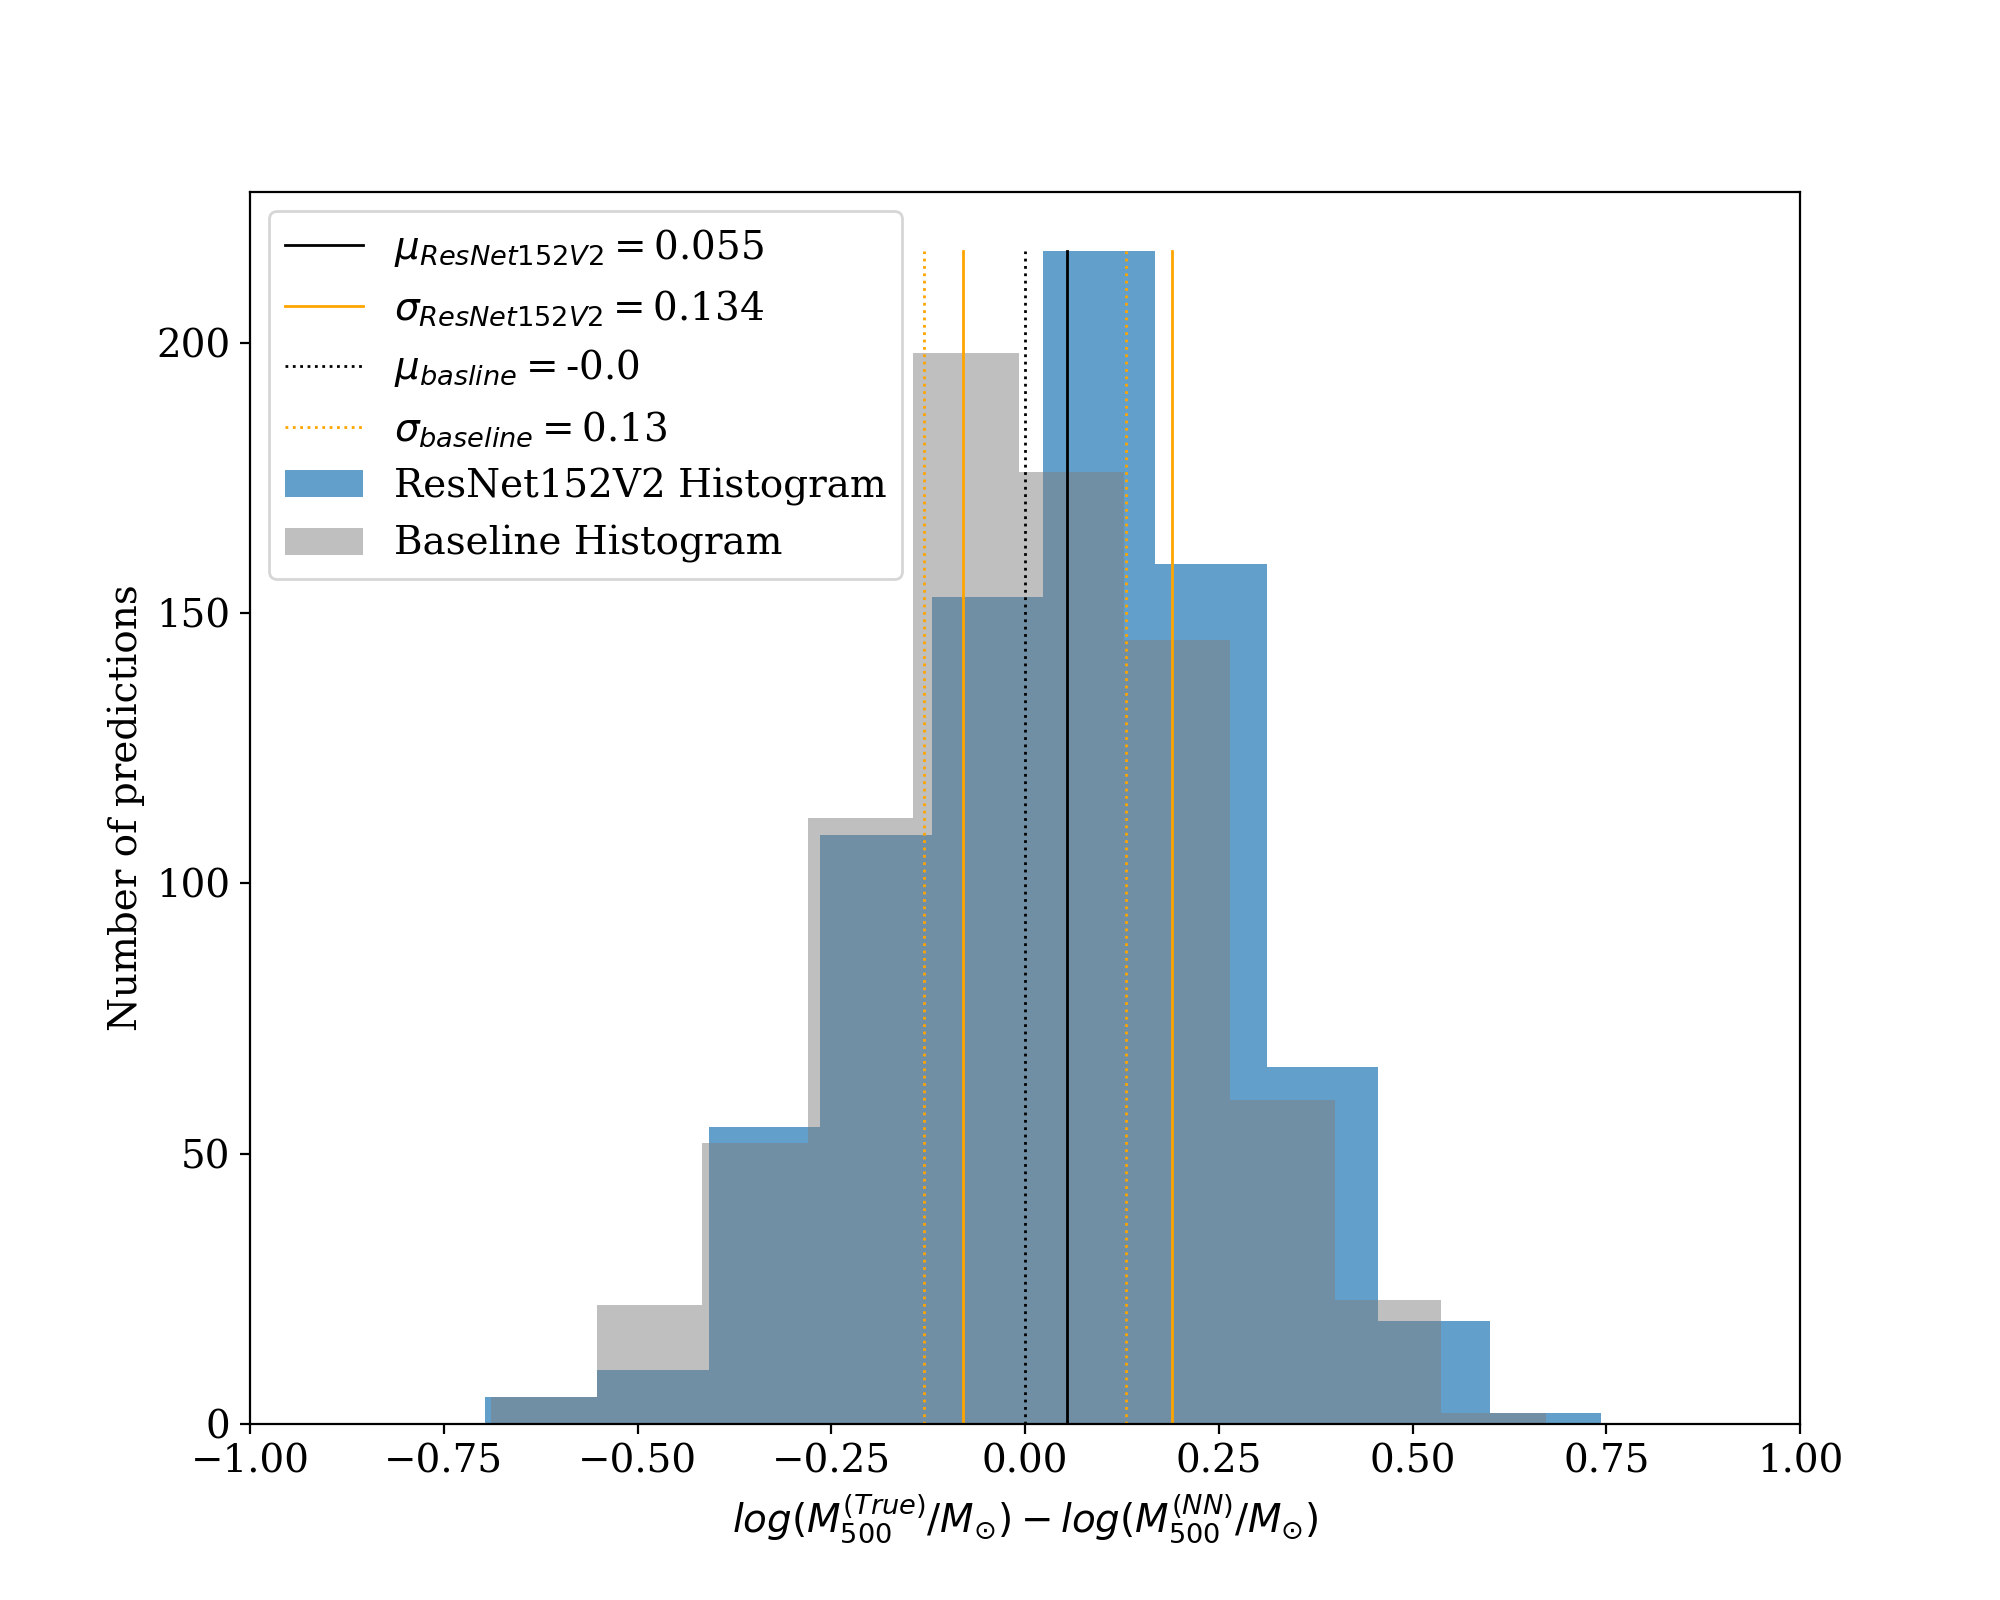
\includegraphics[width=\linewidth]{images/Chapter4/Results/test_ResNet152V2_hist.png}
    \label{fig:test_ResNet152V2_hist}
\end{subfigure}
\label{fig:res52v2_all}
\caption{ResNet152V2 was able to predict almost as accurately as the basic CNN. The deep model's predictions are slightly smaller than the true masses resulting in a positive $\mu$. The basic CNN was able to perform a little bit better in this regard with a $\mu$ of almost zero.}
\end{figure}

\begin{figure}[H]
\begin{subfigure}{.5\textwidth}
    \centering
    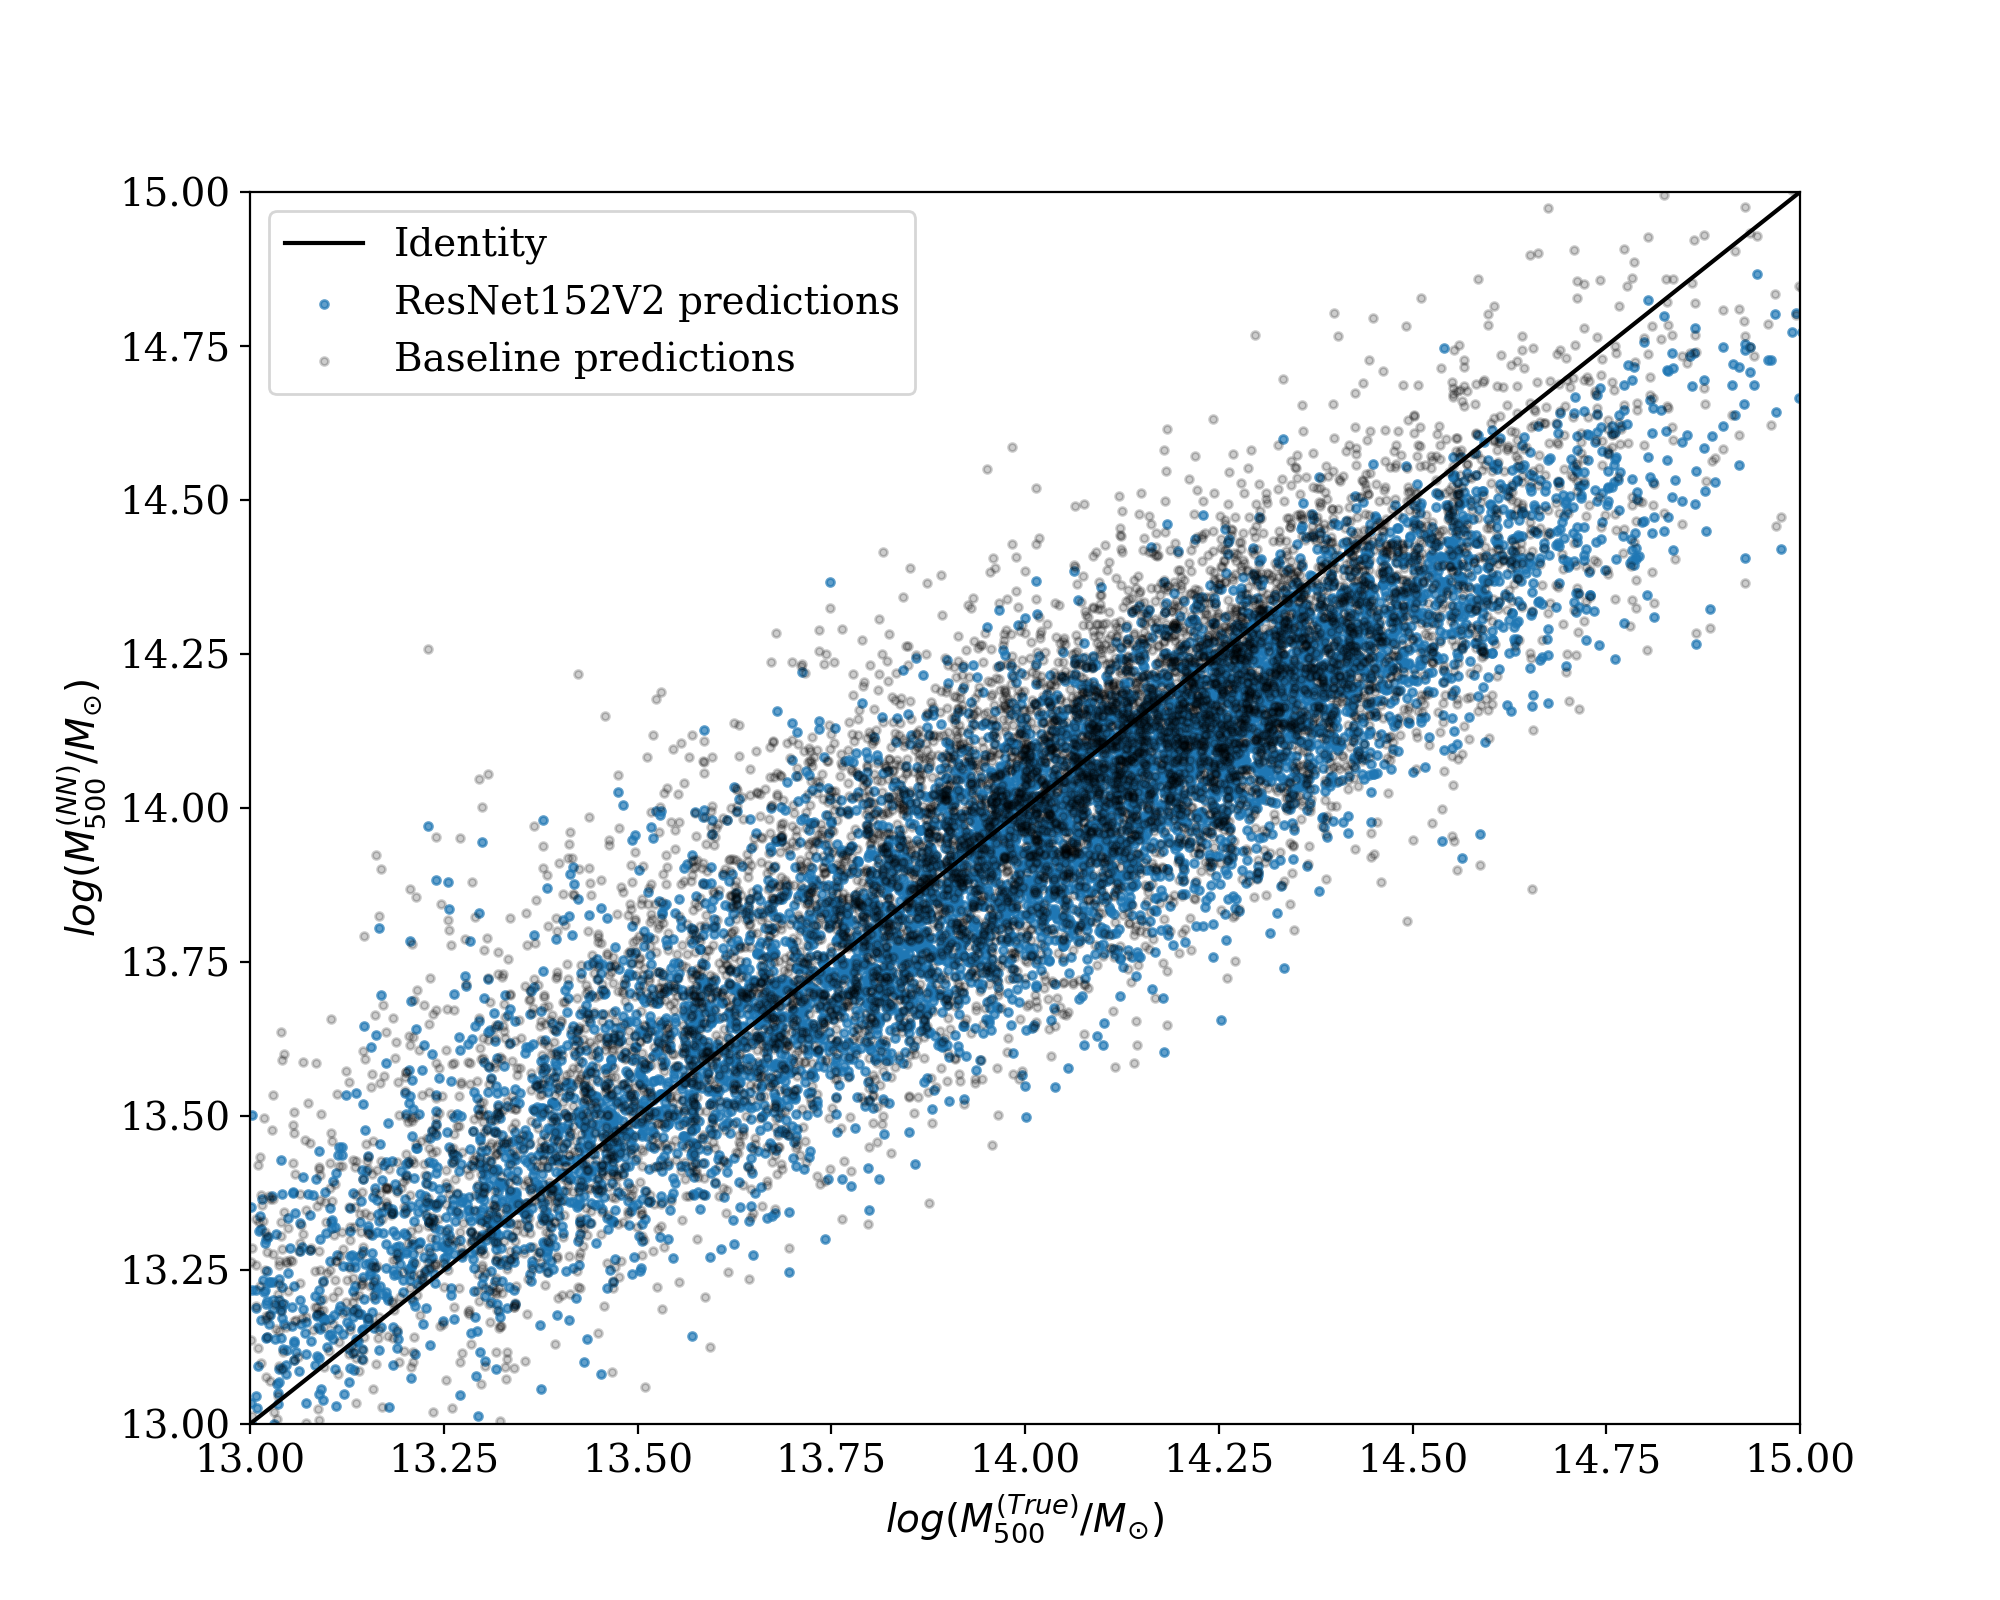
\includegraphics[width=\linewidth]{images/Chapter4/Results/training_ResNet152V2_scatter.png}
    \label{fig:training_ResNet152V2_scatter}
\end{subfigure}
\begin{subfigure}{.5\textwidth}
    \centering
    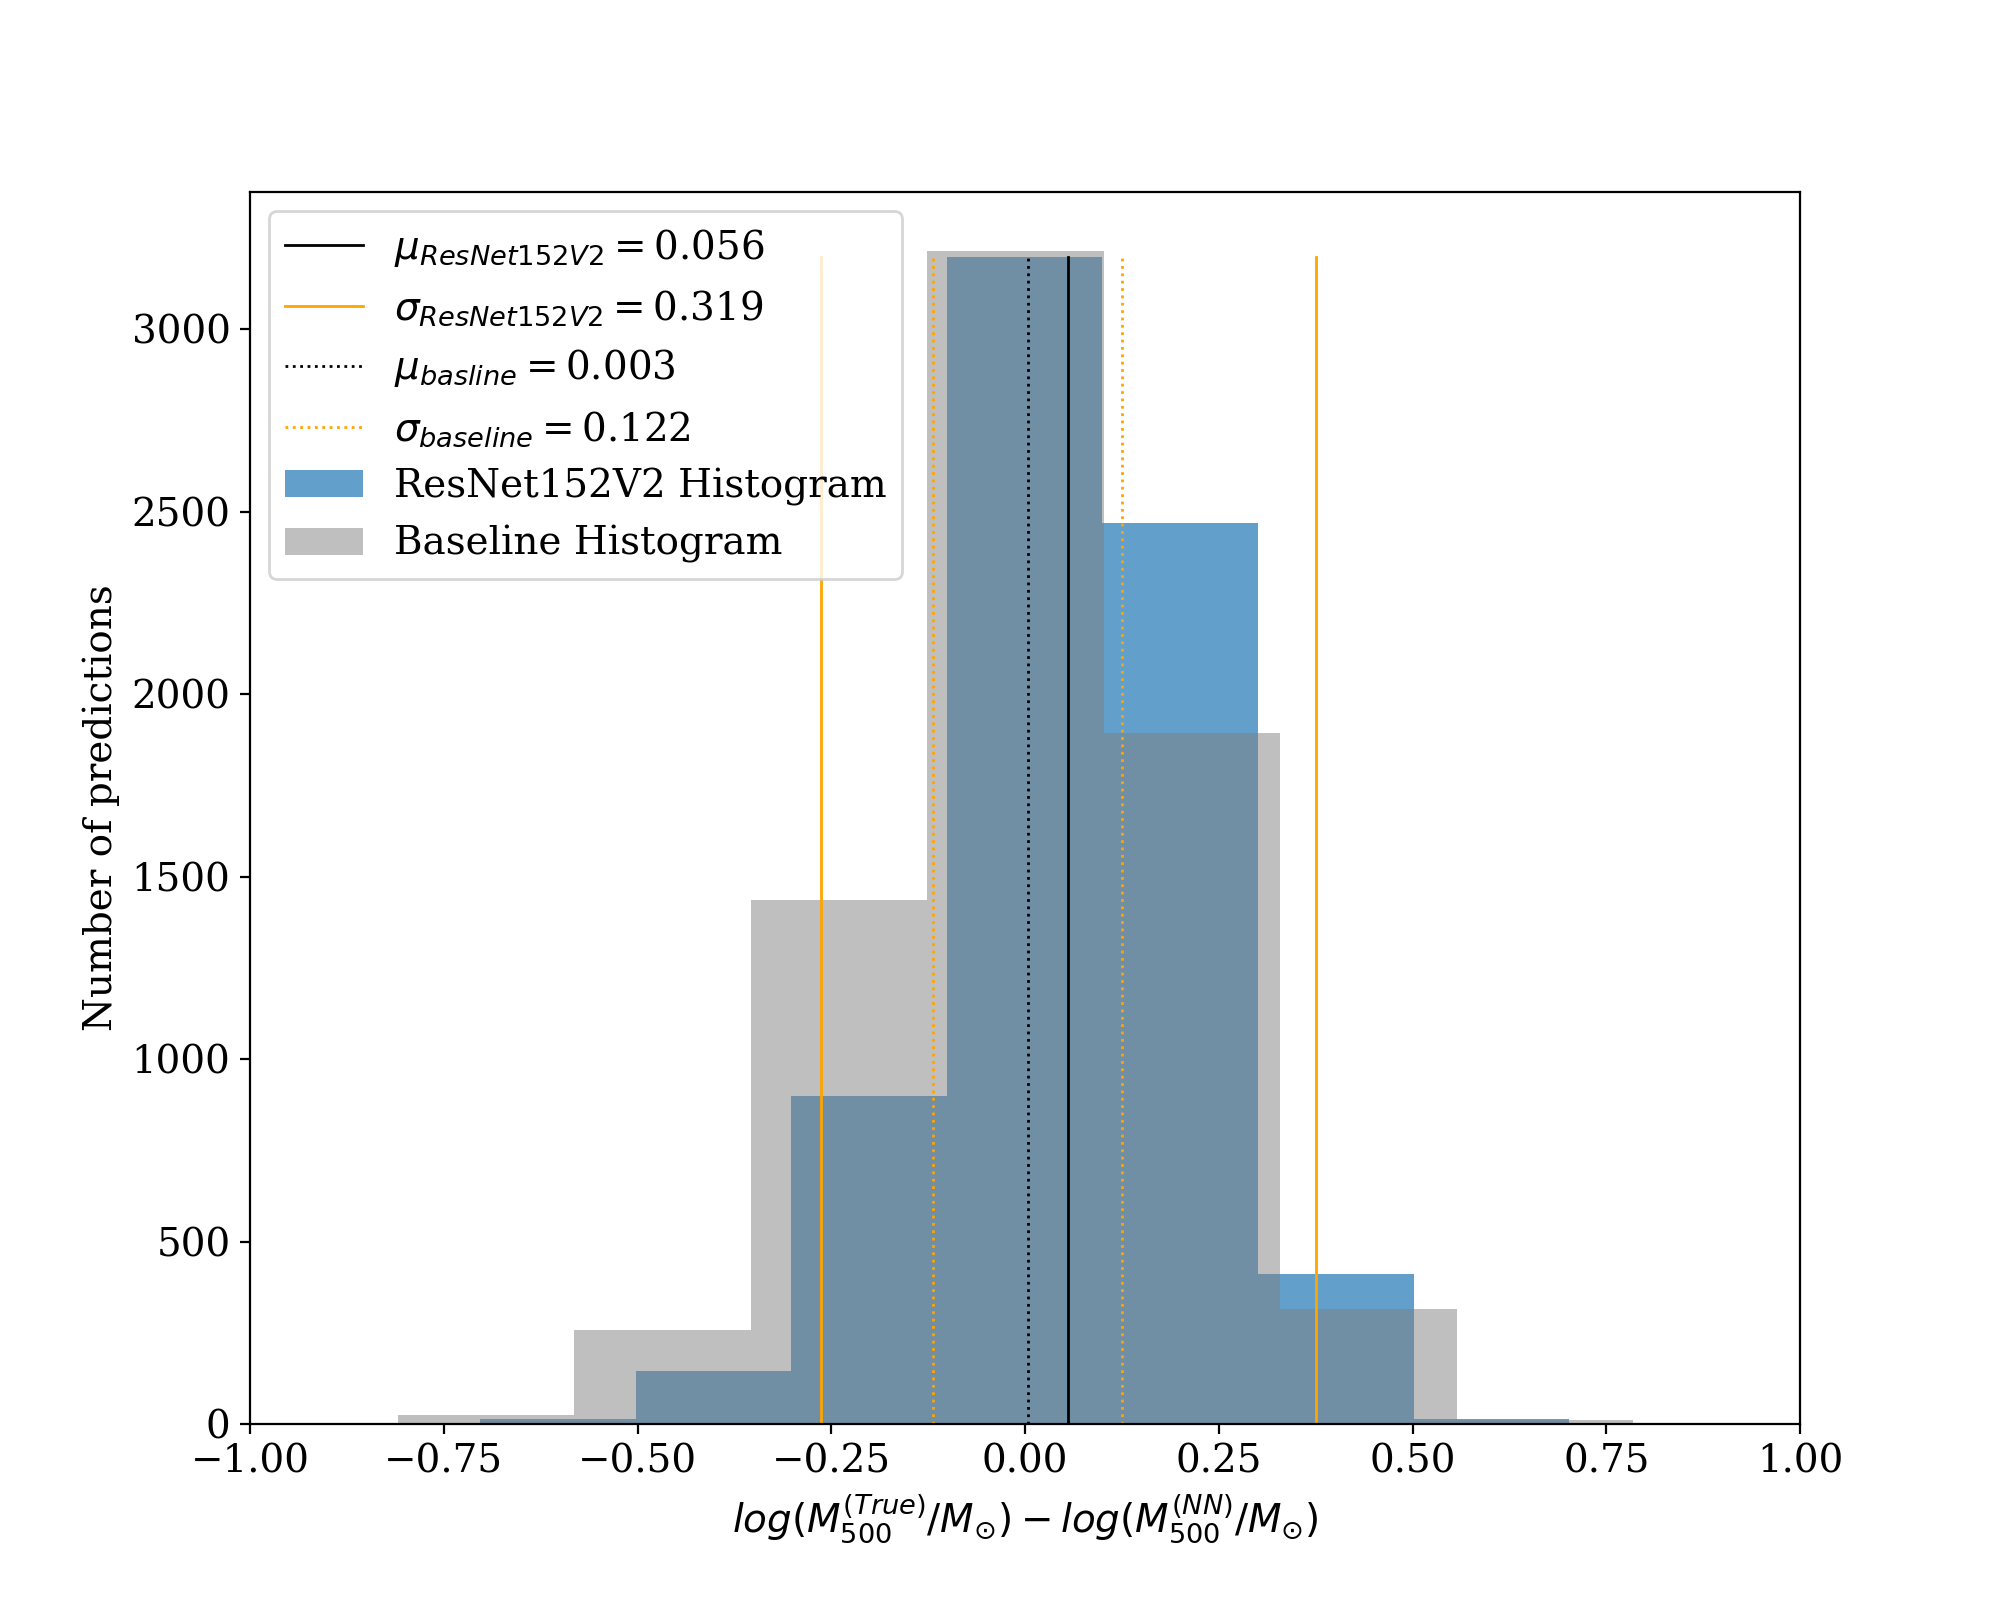
\includegraphics[width=\linewidth]{images/Chapter4/Results/training_ResNet152V2_hist.png}
    \label{fig:training_ResNet152V2_hist}
\end{subfigure}
\label{fig:res52v2_all_training}
\caption{Predictions on the training set look similar too. ResNet152V2 again predicted slightly lower masses than the baseline CNN. The standard deviation $\sigma$ is way bigger for the deep model because of a few very bad fits outside the mass range.}
\end{figure}

All comparison plots between the deep models and the baseline can be found in \cref{app}.\\

Another aspect worth mentioning is the training randomness especially with deep models. I had very different results for ResNet152V2 (and all ResNet models) for every single training run where only one was able to get this close to the basic CNN. The baseline however was able to make accurate predictions in almost every training run with way less randomness and exploding validation losses. This could be caused by the deep model's complexity with over 200 times more trainable parameters (see \autoref{tab:model_params}). This problem could be solved with a careful selection of the learning rate. Even features like a variable learning rate, where the learning rate is changed depending on the model's training, could improve training efficiency for the deep models. This is only one of many ways though to help increase the effectiveness of these long training runs. I will discuss how one could continue with optimization of deep models for galaxy cluster estimation in the conclusion in \cref{conclusion}.

\subsubsection{Table}
For the results of all best performing models consider \autoref{tab:results_table}.
\begin{table*}[h]
\centering
\begin{tabular}{@{}ccccccc@{}}\toprule
Model Name & Training Loss* & Validation Loss* & $\sigma^{\text{test}}$ & $\mu^{\text{test}}$ & $\sigma^{\text{train}}$ & $\mu^{\text{train}}$ \\
\midrule
Basic CNN & $0.046^{\dag}$ & $0.047^{\dag}$ & $0.13$ & $0$ & $0.122$ & $0.003$\\
VGG16 & $0.104$ & $0.102$ & $0.2$ & $-0.019$ & $0.196$ & $-0.027$\\
VGG19 & $0.103$ & $0.102$ & $0.201$ & $0.014$ & $0.195$ & $0.006$ \\
ResNet50 & $0.001$ & $0.09$ & $0.185$ & $-0.035$ & $0.147$& $0.04$\\
ResNet50V2 & $0.0001$ & $0.056$ & $0.14$ & $0.087$ & $0.127$ & $0.087$\\
ResNet101 & $0.0001$ & $0.093$ & $0.182$ & $0.056$ & $0.142$ & $0.055$\\
ResNet101V2 & $0.0001$  &  $0.064$ & $0.148$ & $0.092$ & $0.993$ & $0.092$\\
ResNet152 & $0.0002$ & $0.114$ & $0.201$ & $0.001$ & $0.150$ & $0.017$\\
ResNet152V2 & $0.0001$  & $0.052$ & $0.134$ & $0.055$ & $0.319$ & $0.056$  \\
EfficientNet-B7 &  $0.0002$ & $0.101$ & $0.183$ & $0.037$ & $0.190$ & $0.045$ \\
\bottomrule
\end{tabular}
\caption{Complete training results for the best performing models. It shows how the improved ResNet versions were able to perform better than their predecessors. The VGG and EfficientNet models did not produce accurate results.  *After the last epoch, $^{\dag}$training and validation loss for the epoch with the lowest validation loss value, 15 epochs before the training ended.}
\label{tab:results_table}
\end{table*}






